% IEEE conference format. Compile: pdflatex paper && bibtex paper && pdflatex paper && pdflatex paper
% Every number below is traceable to docs/results/*.csv|json (see paper/REPRODUCIBILITY.md).
\documentclass[conference]{IEEEtran}
\usepackage{graphicx,booktabs,amsmath,cite,url,siunitx}
\sisetup{detect-all}

\begin{document}

\title{How Close Must You Shoot? A Real-Data Study of Image-Resolution Limits \\ for Photo-Based Concrete Crack-Width Measurement}

\author{\IEEEauthorblockN{[Author names and affiliations to be added]}}

\maketitle

\begin{abstract}
Photo-based crack-width measurement is routinely reported in millimetres or below, yet the relation between image
resolution and attainable accuracy on real concrete cracks is rarely quantified. We study this relation using
14{,}198 real brightness profiles across cracks (0.004--0.81~mm; 9\,\% below 0.05~mm) from the open krkCMd dataset, each with a manual
reference width. Profiles are re-imaged at 2.5--252~px/mm under two imaging scenarios (ideal scan and a
phone-like blur/noise model), and widths are measured with a sub-pixel full-width-at-half-maximum (FWHM)
estimator and two classical baselines. Mean absolute error is flat at about \SI{56}{\micro\metre} down to
25~px/mm, then rises steeply: \SI{141}{\micro\metre} at 8~px/mm and \SI{423}{\micro\metre} at 3.6~px/mm, the
latter worse than predicting the dataset's mean width (\SI{112}{\micro\metre}). A two-parameter-family model,
$\mathrm{MAE}(p)=a+c\,p^{k}$ in the pixel pitch $p$, fits the curve (pooled RMSE \SI{9}{\micro\metre}) and
predicts held-out specimen series within 23--33\,\%. An end-to-end 2-D experiment with segmentation and
skeletonisation on held-out specimens confirms the trend. Cracks of 0.04~mm are not measurable by profile-width methods even at
252~px/mm in this data. We translate the model into a camera-distance planning rule and release code,
tables and a printable test chart for independent validation with real cameras.
\end{abstract}

\begin{IEEEkeywords}
crack width, concrete, image resolution, measurement uncertainty, structural health monitoring, sub-pixel measurement
\end{IEEEkeywords}

\section{Introduction}
Visual inspection of concrete is increasingly supported by photographs from handheld cameras and drones, and many
pipelines output a crack width in millimetres. Segmentation networks for cracks are well studied
\cite{liu2019deepcrack,ronneberger2015unet,dorafshan2018sdnet,ozgenel2018isarc}, but the \emph{metrological} question---how
precisely can a width be read from a photo of a given ground sampling distance---is much less often answered with
real, independently referenced cracks. Practitioners therefore lack a defensible rule for how close to
photograph a crack of a given width.

This paper makes three contributions:
\begin{enumerate}
\item A real-data resolution study of photo-based crack-width measurement on 14{,}198 reference-annotated crack profiles, with baselines, bootstrap confidence intervals, a no-skill reference and leave-one-specimen-series-out validation.
\item A compact predictive error model and a camera-distance planner derived from it, including an explicit statement of when a measurement carries no information beyond the dataset mean.
\item An open, reproducible toolchain: measurement code, evaluation scripts, a printable known-width test chart with analysis software, and a range-request fetcher for the 38~GB source images.
\end{enumerate}
We state limitations prominently (Section~\ref{sec:limits}); in particular our measurement is \emph{not} more accurate than the dataset's own deep-learning
benchmark, and we make no state-of-the-art claim.

\section{Related Work}
Crack segmentation benchmarks and models \cite{liu2019deepcrack,dorafshan2018sdnet,ozgenel2018isarc,ronneberger2015unet} focus on detection
and pixel masks. Thin dark curvilinear structures are classically enhanced with multi-scale Hessian line filters
\cite{sato1998line,frangi1998vessel}, which we use for a training-free segmentation baseline; global thresholding is represented
by Otsu's method \cite{otsu1979threshold}. The krkCMd dataset \cite{jakubowski2025krkcmd} provides, uniquely, sub-0.1~mm to 0.8~mm
crack profiles with a manual reference width and benchmark estimates from a deep-learning metasensor and an edge detector; we build on it.

\section{Methods}
\subsection{Data}
krkCMd comprises scanner images (pixel pitch \SI{3.97}{\micro\metre}, about 252~px/mm) of self-healing concrete specimens in four series
(w/c 0.23 and 0.28; 2 and 20 months), with 501-pixel brightness profiles across the crack and a manual width reference
(one trained operator, steepest-edge marking, bevelled edges excluded) \cite{jakubowski2025krkcmd}. Profiles with reference width zero (fully healed) are excluded,
leaving $n=14{,}198$. The data are CC~BY~4.0.

\subsection{Imaging simulation}
Each profile is re-imaged at a target resolution $r\in\{252,100,50,25,12.5,8,5,3.6,2.5\}$~px/mm: optional Gaussian optical
PSF, integration over square pixels of pitch $p=1000/r~\mu$m with a random sub-pixel phase, additive Gaussian noise and 8-bit
quantisation. Two scenarios are used: \emph{ideal scan} (no PSF, $\sigma_n=2$ grey levels) and \emph{phone-like}
(PSF $\sigma=0.7$~px, $\sigma_n=4$). The measurement window is fixed at $\pm0.8$~mm and independent of the true width.

\subsection{Width estimators}
\emph{Sub-pixel FWHM} (ours): the image is smoothed ($\sigma=0.8$~px), the dark dip's half-depth crossings are located with linear interpolation, and the
smoothing's FWHM is removed in quadrature. \emph{Threshold count}: pixels below the half-depth level counted with no interpolation.
\emph{Gradient edges}: distance between the steepest descending and ascending edge (parabolic refinement), mirroring how the reference was marked.
We additionally report the dataset's own estimators (deep-learning metasensor and threshold edge detector) at native resolution.

\subsection{Error model, calibration, no-skill reference}
We fit $\mathrm{MAE}(p)=a+c\,p^{k}$ to per-series error curves and validate leave-one-series-out. A linear calibration
$w_\mathrm{ref}\approx \alpha w_\mathrm{meas}+\beta$ is likewise fitted on three series and applied to the fourth. The \emph{no-skill}
reference always predicts the mean reference width of the other series.

\subsection{End-to-end 2-D evaluation}
Image bands (full-width horizontal strips covering all annotated gridlines, retrieved with HTTP range requests) are re-imaged as above, segmented
(multi-scale Sato ridge filter with shape filtering, or flattened Otsu), skeletonised and measured with the same FWHM routine at skeleton points within 0.3~mm
of each annotated crack centre; otherwise the gridline is a miss. Ridge hyper-parameters were tuned on the development series only and frozen for the held-out series.

\section{Results}
\subsection{Resolution dependence (1-D study)}
Table~\ref{tab:mae} and Fig.~\ref{fig:mae} give mean absolute error against resolution in the phone-like scenario (bootstrap 95\,\% CIs over profiles are
within $\pm$2\,\% of the means; \texttt{mae\_bootstrap\_ci.csv}). Error is flat (about \SI{56}{\micro\metre}) from 252 to 50~px/mm and rises below about
25~px/mm. Sub-pixel interpolation gives a 21\,\% lower MAE than threshold counting at 2.5~px/mm and 12\,\% at 3.6~px/mm, and no gain at $\geq$8~px/mm.

\begin{table}[t]
\centering\caption{Mean absolute error ($\mu$m), phone-like imaging, 14{,}198 profiles.}\label{tab:mae}
\begin{tabular}{rrrr}
\toprule
px/mm & Sub-pixel FWHM & Threshold & Gradient edges\\
\midrule
252 & 56 & 55 & 69\\
50 & 57 & 59 & 71\\
25 & 61 & 65 & 82\\
12.5 & 86 & 91 & 135\\
8 & 141 & 142 & 238\\
5 & 271 & 279 & 454\\
3.6 & 423 & 482 & 707\\
2.5 & 701 & 887 & 1153\\
\bottomrule
\end{tabular}
\end{table}

\begin{figure}[t]
\centering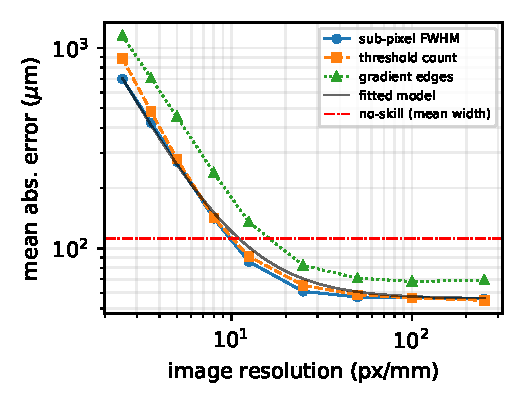
\includegraphics[width=\columnwidth]{figures/fig_mae_vs_resolution.pdf}
\caption{MAE versus resolution with fitted model $a+c\,p^k$ and the no-skill level (\SI{112}{\micro\metre}).}\label{fig:mae}
\end{figure}

\subsection{Width-dependent resolvability}
Fig.~\ref{fig:heat} shows the median relative error by true-width bin and resolution (phone-like). A 200--400~$\mu$m crack stays within about 14\,\% down to 12.5~px/mm and 25\,\%
at 8~px/mm; 100--200~$\mu$m requires $\geq$25~px/mm for about 24\,\%; 50--100~$\mu$m is about 48\,\% even at 252~px/mm; cracks under 50~$\mu$m exceed 130\,\% at every resolution.

\begin{figure}[t]
\centering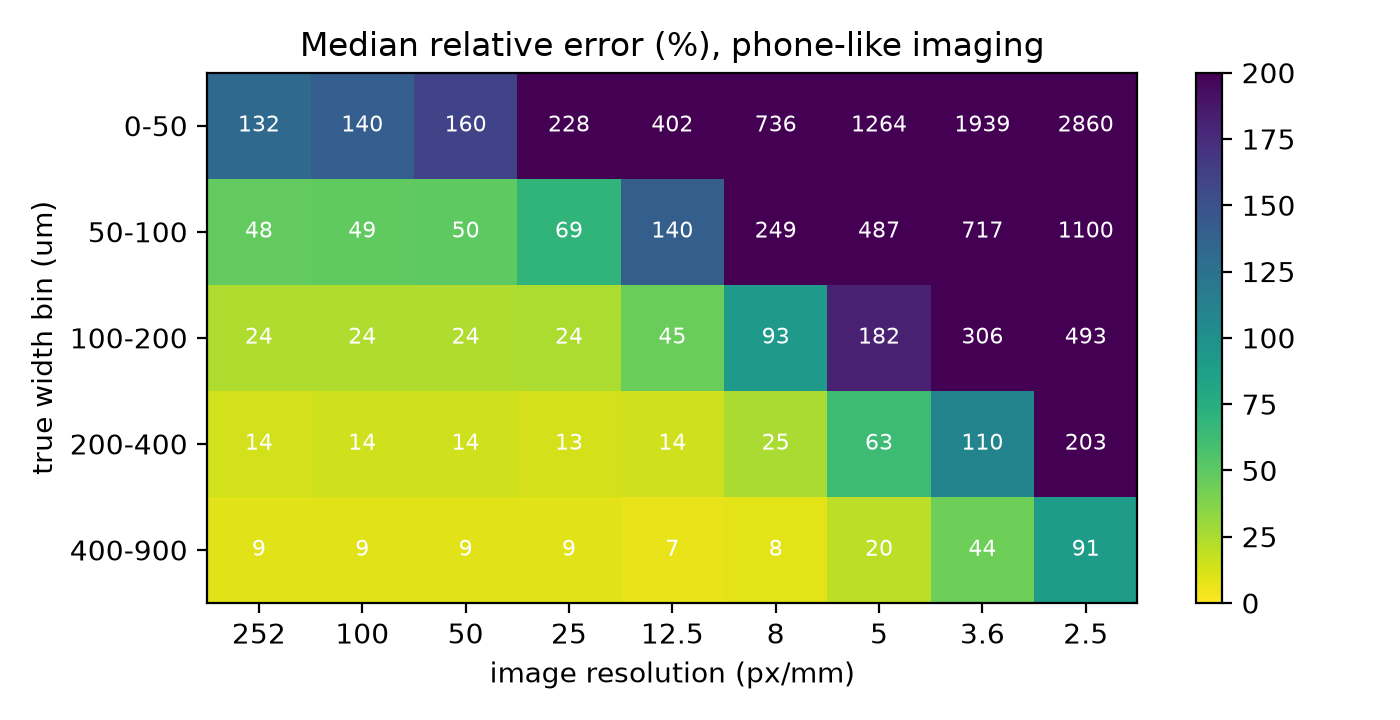
\includegraphics[width=\columnwidth]{figures/fig_error_heatmap.png}
\caption{Median relative error (\%) by true width and resolution, phone-like imaging.}\label{fig:heat}
\end{figure}

\subsection{Systematic offset, calibration and comparison with dataset benchmarks}
All three profile-based estimators carry a roughly constant positive bias of \SI{55}{\micro\metre} at $\geq$25~px/mm (stage-wise $+72$ to $+45$~$\mu$m).
It is a definitional offset between half-depth FWHM and the operator's steepest-edge marking, not noise. Leave-one-series-out linear calibration reduces MAE to
\SI{37}{\micro\metre} at 252~px/mm and \SI{47}{\micro\metre} at 25~px/mm, but only to \SI{98}{\micro\metre} at 8~px/mm and \SI{112}{\micro\metre} at 3.6~px/mm, i.e.\ the
no-skill level. For reference, the dataset's own deep-learning metasensor and edge detector reach MAE \SI{14.9}{\micro\metre} and \SI{38.0}{\micro\metre} at native resolution; our
estimator is not competitive with the former.

\subsection{Predictive model and planning rule}
The fit is $\mathrm{MAE}(p)=56.0+0.0324\,p^{1.65}$~$\mu$m (pooled RMSE \SI{8.8}{\micro\metre}); leave-one-series-out prediction errors are 23--33\,\% of the measured MAE.
Inverting the model with a pinhole camera model $r=f/(D\,s)$ gives a planning rule. For example, for a $\pm25$\,\% tolerance on a 0.3~mm crack the uncalibrated estimator needs
$\geq$21~px/mm, i.e.\ a camera distance of at most 20~cm for a 6.0~mm focal length and 1.4~$\mu$m pixels; for 0.5~mm, $\geq$9.7~px/mm (44~cm). A $\pm25$\,\% tolerance on
0.1--0.2~mm is below the uncalibrated error floor. After calibration the planner reports $\geq$47~px/mm for 0.2~mm, but at coarse resolution calibrated performance approaches the
no-skill level, so such outputs only assert that the measurement is informative, not that a specific crack is read correctly.

\subsection{End-to-end 2-D results}
Table~\ref{tab:2d} gives phone-like results on the development (tuned) and held-out specimen series. Hit rates are about 100\,\% down to 8~px/mm for both segmenters; error trends match the 1-D study
(8~px/mm: \SI{174}{\micro\metre} held-out versus \SI{141}{\micro\metre} in 1-D) with larger absolute bias on these two wide-crack stages. The ridge filter is not better than Otsu on these clean laboratory surfaces.

\begin{table}[t]
\centering\caption{End-to-end MAE ($\mu$m) and hit rate, phone-like imaging (161 dev / 254 held-out gridlines).}\label{tab:2d}
\begin{tabular}{rrrr}
\toprule
px/mm & Ridge (held-out) & Otsu (held-out) & Ridge (dev)\\
\midrule
50 & 97 (1.00) & 118 (1.00) & 117 (1.00)\\
25 & 96 (1.00) & 103 (1.00) & 116 (1.00)\\
12.5 & 115 (1.00) & 114 (1.00) & 129 (0.99)\\
8 & 174 (1.00) & 186 (1.00) & 166 (0.99)\\
5 & 273 (0.98) & 308 (1.00) & 255 (0.97)\\
3.6 & 405 (0.88) & 475 (1.00) & 381 (0.93)\\
\bottomrule
\end{tabular}
\end{table}

\begin{figure}[t]
\centering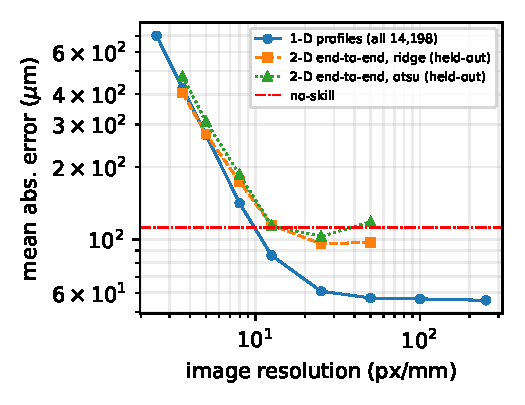
\includegraphics[width=\columnwidth]{figures/fig_1d_vs_2d.pdf}
\caption{1-D study versus end-to-end 2-D (held-out series), phone-like imaging.}\label{fig:2d}
\end{figure}

\section{Discussion}
The practical message is that the \emph{sampling density}, not the segmentation network, bounds crack-width accuracy in laboratory-quality images. Below about 8--12~px/mm, a
reported width is no more informative than the typical width of the population. For a typical phone photograph of a drill core (3--4~px/mm) the expected error is roughly 0.4~mm,
larger than most cracks that matter for durability limits. Hairline cracks near 0.04~mm are out of reach for profile-width estimators, including at 252~px/mm in this data, where
the offset between measurement definitions and the reference's own precision dominate.

\section{Limitations and Threats to Validity}\label{sec:limits}
\begin{itemize}
\item \textbf{Reference.} A single operator's manual widths, not a physical gauge; reference uncertainty is unquantified and may limit conclusions below $\sim$0.1~mm.
\item \textbf{Simulated lower resolution.} Coarse images are synthesised from scanner data; they are not real phone photographs of rough surfaces under field lighting. A known-width printed chart and analysis code are provided for the real-camera experiment, which we have not yet run on physical prints.
\item \textbf{Scope and sample.} Four specimen series from one laboratory; the 2-D study uses one image per series at two stages (415 gridlines) with no confidence intervals.
\item \textbf{Bias.} A $\sim$55~$\mu$m definitional offset dominates the uncalibrated error at fine resolution and varies across stages; a single global calibration is imperfect.
\item \textbf{Model extrapolation.} The error model is fitted on cracks of 0.004--0.81~mm and does not extrapolate to wider cracks or field conditions. The calibrated fit's coarse-resolution behaviour reflects regression to the mean.
\item \textbf{Competitiveness.} The dataset's own deep-learning benchmark is more accurate than our estimator; the contribution is characterisation, not a new estimator.
\end{itemize}

\section{Conclusion and Future Work}
On real concrete cracks, the accuracy of photo-based width measurement is governed by image resolution through a simple, validated relation, and below roughly 8--12~px/mm a
width estimate carries little information beyond the population mean. Future work: (i) run the printed-chart study with real cameras and calibrated line widths, (ii) extend the 2-D study to all 36 images and add confidence intervals,
(iii) add cluttered field photographs, and (iv) compare against published learning-based width estimators on the same protocol.

\section*{Data and Code Availability}
krkCMd: Zenodo \texttt{10.5281/zenodo.14568863} (CC~BY~4.0). Code, result tables and the test chart: project repository (to be archived with a DOI at submission).

\bibliographystyle{IEEEtran}
\bibliography{references}
\end{document}
